% The Tokenizer Tax -- 4-page ACL short paper (draft). Owner: Saket (lane A).
% Overleaf: start from the official ACL template (acl.sty / acl_natbib.bst from github.com/acl-org/acl-style-files),
% then drop in this file, refs.bib, numbers.tex and ../figures/*.pdf.
% Every number comes from numbers.tex (scripts/make_paper_numbers.py). Never type a result by hand.
\documentclass[11pt]{article}
\usepackage[review]{acl}
\usepackage[T1]{fontenc}
\usepackage[utf8]{inputenc}
\usepackage{microtype}
\usepackage{amsmath,amssymb}
\usepackage{graphicx}
\usepackage{booktabs}
\graphicspath{{../figures/}{figures/}}
% AUTO-GENERATED by scripts/make_paper_numbers.py -- do not edit by hand
\newcommand{\taxClAsm}{6.3}
\newcommand{\fertClAsm}{8.82}
\newcommand{\fertratioClAsm}{7.1}
\newcommand{\sbClAsm}{90}
\newcommand{\inrClAsm}{7.37}
\newcommand{\taxClBen}{5.9}
\newcommand{\fertClBen}{8.20}
\newcommand{\fertratioClBen}{6.6}
\newcommand{\sbClBen}{85}
\newcommand{\inrClBen}{6.93}
\newcommand{\taxClEng}{1.0}
\newcommand{\fertClEng}{1.24}
\newcommand{\fertratioClEng}{1.0}
\newcommand{\sbClEng}{0}
\newcommand{\inrClEng}{1.18}
\newcommand{\taxClGuj}{7.7}
\newcommand{\fertClGuj}{9.97}
\newcommand{\fertratioClGuj}{8.0}
\newcommand{\sbClGuj}{98}
\newcommand{\inrClGuj}{9.02}
\newcommand{\taxClHin}{4.8}
\newcommand{\fertClHin}{5.05}
\newcommand{\fertratioClHin}{4.1}
\newcommand{\sbClHin}{61}
\newcommand{\inrClHin}{5.61}
\newcommand{\taxClKan}{8.9}
\newcommand{\fertClKan}{14.95}
\newcommand{\fertratioClKan}{12.0}
\newcommand{\sbClKan}{98}
\newcommand{\inrClKan}{10.43}
\newcommand{\taxClMal}{8.9}
\newcommand{\fertClMal}{16.27}
\newcommand{\fertratioClMal}{13.1}
\newcommand{\sbClMal}{97}
\newcommand{\inrClMal}{10.53}
\newcommand{\taxClMar}{5.0}
\newcommand{\fertClMar}{7.21}
\newcommand{\fertratioClMar}{5.8}
\newcommand{\sbClMar}{68}
\newcommand{\inrClMar}{5.95}
\newcommand{\taxClOri}{12.4}
\newcommand{\fertClOri}{17.23}
\newcommand{\fertratioClOri}{13.9}
\newcommand{\sbClOri}{99}
\newcommand{\inrClOri}{14.65}
\newcommand{\taxClPan}{7.9}
\newcommand{\fertClPan}{8.32}
\newcommand{\fertratioClPan}{6.7}
\newcommand{\sbClPan}{99}
\newcommand{\inrClPan}{9.34}
\newcommand{\taxClTam}{7.6}
\newcommand{\fertClTam}{12.39}
\newcommand{\fertratioClTam}{10.0}
\newcommand{\sbClTam}{89}
\newcommand{\inrClTam}{9.00}
\newcommand{\taxClTel}{8.3}
\newcommand{\fertClTel}{13.30}
\newcommand{\fertratioClTel}{10.7}
\newcommand{\sbClTel}{98}
\newcommand{\inrClTel}{9.76}
\newcommand{\taxClUrd}{4.3}
\newcommand{\fertClUrd}{4.27}
\newcommand{\fertratioClUrd}{3.4}
\newcommand{\sbClUrd}{34}
\newcommand{\inrClUrd}{5.11}
\newcommand{\taxGeAsm}{3.2}
\newcommand{\fertGeAsm}{4.48}
\newcommand{\fertratioGeAsm}{3.6}
\newcommand{\sbGeAsm}{0}
\newcommand{\taxGeBen}{2.7}
\newcommand{\fertGeBen}{3.70}
\newcommand{\fertratioGeBen}{3.0}
\newcommand{\sbGeBen}{0}
\newcommand{\taxGeEng}{1.0}
\newcommand{\fertGeEng}{1.23}
\newcommand{\fertratioGeEng}{1.0}
\newcommand{\sbGeEng}{0}
\newcommand{\taxGeGuj}{3.0}
\newcommand{\fertGeGuj}{3.90}
\newcommand{\fertratioGeGuj}{3.2}
\newcommand{\sbGeGuj}{0}
\newcommand{\taxGeHin}{1.9}
\newcommand{\fertGeHin}{1.96}
\newcommand{\fertratioGeHin}{1.6}
\newcommand{\sbGeHin}{0}
\newcommand{\taxGeKan}{3.3}
\newcommand{\fertGeKan}{5.55}
\newcommand{\fertratioGeKan}{4.5}
\newcommand{\sbGeKan}{0}
\newcommand{\taxGeMal}{3.2}
\newcommand{\fertGeMal}{5.87}
\newcommand{\fertratioGeMal}{4.8}
\newcommand{\sbGeMal}{0}
\newcommand{\taxGeMar}{2.3}
\newcommand{\fertGeMar}{3.20}
\newcommand{\fertratioGeMar}{2.6}
\newcommand{\sbGeMar}{0}
\newcommand{\taxGeOri}{5.0}
\newcommand{\fertGeOri}{6.86}
\newcommand{\fertratioGeOri}{5.6}
\newcommand{\sbGeOri}{0}
\newcommand{\taxGePan}{3.2}
\newcommand{\fertGePan}{3.38}
\newcommand{\fertratioGePan}{2.7}
\newcommand{\sbGePan}{0}
\newcommand{\taxGeTam}{2.6}
\newcommand{\fertGeTam}{4.19}
\newcommand{\fertratioGeTam}{3.4}
\newcommand{\sbGeTam}{0}
\newcommand{\taxGeTel}{2.9}
\newcommand{\fertGeTel}{4.57}
\newcommand{\fertratioGeTel}{3.7}
\newcommand{\sbGeTel}{0}
\newcommand{\taxGeUrd}{1.9}
\newcommand{\fertGeUrd}{1.89}
\newcommand{\fertratioGeUrd}{1.5}
\newcommand{\sbGeUrd}{0}
\newcommand{\taxOoAsm}{2.0}
\newcommand{\fertOoAsm}{2.78}
\newcommand{\fertratioOoAsm}{2.3}
\newcommand{\sbOoAsm}{1}
\newcommand{\inrOoAsm}{0.58}
\newcommand{\taxOoBen}{1.7}
\newcommand{\fertOoBen}{2.36}
\newcommand{\fertratioOoBen}{1.9}
\newcommand{\sbOoBen}{1}
\newcommand{\inrOoBen}{0.50}
\newcommand{\taxOoEng}{1.0}
\newcommand{\fertOoEng}{1.23}
\newcommand{\fertratioOoEng}{1.0}
\newcommand{\sbOoEng}{0}
\newcommand{\inrOoEng}{0.29}
\newcommand{\taxOoGuj}{1.8}
\newcommand{\fertOoGuj}{2.30}
\newcommand{\fertratioOoGuj}{1.9}
\newcommand{\sbOoGuj}{2}
\newcommand{\inrOoGuj}{0.52}
\newcommand{\taxOoHin}{1.6}
\newcommand{\fertOoHin}{1.65}
\newcommand{\fertratioOoHin}{1.3}
\newcommand{\sbOoHin}{0}
\newcommand{\inrOoHin}{0.46}
\newcommand{\taxOoKan}{2.0}
\newcommand{\fertOoKan}{3.28}
\newcommand{\fertratioOoKan}{2.7}
\newcommand{\sbOoKan}{1}
\newcommand{\inrOoKan}{0.57}
\newcommand{\taxOoMal}{2.0}
\newcommand{\fertOoMal}{3.52}
\newcommand{\fertratioOoMal}{2.9}
\newcommand{\sbOoMal}{2}
\newcommand{\inrOoMal}{0.57}
\newcommand{\taxOoMar}{1.8}
\newcommand{\fertOoMar}{2.56}
\newcommand{\fertratioOoMar}{2.1}
\newcommand{\sbOoMar}{1}
\newcommand{\inrOoMar}{0.53}
\newcommand{\taxOoOri}{5.0}
\newcommand{\fertOoOri}{6.84}
\newcommand{\fertratioOoOri}{5.6}
\newcommand{\sbOoOri}{27}
\newcommand{\inrOoOri}{1.45}
\newcommand{\taxOoPan}{2.6}
\newcommand{\fertOoPan}{2.72}
\newcommand{\fertratioOoPan}{2.2}
\newcommand{\sbOoPan}{5}
\newcommand{\inrOoPan}{0.76}
\newcommand{\taxOoTam}{2.0}
\newcommand{\fertOoTam}{3.17}
\newcommand{\fertratioOoTam}{2.6}
\newcommand{\sbOoTam}{1}
\newcommand{\inrOoTam}{0.58}
\newcommand{\taxOoTel}{1.9}
\newcommand{\fertOoTel}{3.06}
\newcommand{\fertratioOoTel}{2.5}
\newcommand{\sbOoTel}{4}
\newcommand{\inrOoTel}{0.56}
\newcommand{\taxOoUrd}{1.7}
\newcommand{\fertOoUrd}{1.61}
\newcommand{\fertratioOoUrd}{1.3}
\newcommand{\sbOoUrd}{0}
\newcommand{\inrOoUrd}{0.48}
\newcommand{\taxQwAsm}{5.4}
\newcommand{\fertQwAsm}{7.71}
\newcommand{\fertratioQwAsm}{6.1}
\newcommand{\sbQwAsm}{73}
\newcommand{\inrQwAsm}{0.19}
\newcommand{\taxQwBen}{5.0}
\newcommand{\fertQwBen}{7.12}
\newcommand{\fertratioQwBen}{5.6}
\newcommand{\sbQwBen}{68}
\newcommand{\inrQwBen}{0.18}
\newcommand{\taxQwEng}{1.0}
\newcommand{\fertQwEng}{1.26}
\newcommand{\fertratioQwEng}{1.0}
\newcommand{\sbQwEng}{0}
\newcommand{\inrQwEng}{0.04}
\newcommand{\taxQwGuj}{6.7}
\newcommand{\fertQwGuj}{8.91}
\newcommand{\fertratioQwGuj}{7.1}
\newcommand{\sbQwGuj}{86}
\newcommand{\inrQwGuj}{0.24}
\newcommand{\taxQwHin}{4.4}
\newcommand{\fertQwHin}{4.76}
\newcommand{\fertratioQwHin}{3.8}
\newcommand{\sbQwHin}{51}
\newcommand{\inrQwHin}{0.16}
\newcommand{\taxQwKan}{6.9}
\newcommand{\fertQwKan}{11.87}
\newcommand{\fertratioQwKan}{9.4}
\newcommand{\sbQwKan}{71}
\newcommand{\inrQwKan}{0.25}
\newcommand{\taxQwMal}{7.2}
\newcommand{\fertQwMal}{13.37}
\newcommand{\fertratioQwMal}{10.6}
\newcommand{\sbQwMal}{74}
\newcommand{\inrQwMal}{0.26}
\newcommand{\taxQwMar}{4.6}
\newcommand{\fertQwMar}{6.69}
\newcommand{\fertratioQwMar}{5.3}
\newcommand{\sbQwMar}{58}
\newcommand{\inrQwMar}{0.17}
\newcommand{\taxQwOri}{9.7}
\newcommand{\fertQwOri}{13.65}
\newcommand{\fertratioQwOri}{10.8}
\newcommand{\sbQwOri}{98}
\newcommand{\inrQwOri}{0.35}
\newcommand{\taxQwPan}{7.3}
\newcommand{\fertQwPan}{7.76}
\newcommand{\fertratioQwPan}{6.2}
\newcommand{\sbQwPan}{91}
\newcommand{\inrQwPan}{0.26}
\newcommand{\taxQwTam}{6.1}
\newcommand{\fertQwTam}{10.06}
\newcommand{\fertratioQwTam}{8.0}
\newcommand{\sbQwTam}{63}
\newcommand{\inrQwTam}{0.22}
\newcommand{\taxQwTel}{7.0}
\newcommand{\fertQwTel}{11.40}
\newcommand{\fertratioQwTel}{9.0}
\newcommand{\sbQwTel}{81}
\newcommand{\inrQwTel}{0.25}
\newcommand{\taxQwUrd}{3.1}
\newcommand{\fertQwUrd}{3.14}
\newcommand{\fertratioQwUrd}{2.5}
\newcommand{\sbQwUrd}{0}
\newcommand{\inrQwUrd}{0.11}
\newcommand{\taxSaAsm}{2.8}
\newcommand{\fertSaAsm}{4.50}
\newcommand{\fertratioSaAsm}{3.1}
\newcommand{\sbSaAsm}{39}
\newcommand{\taxSaBen}{1.1}
\newcommand{\fertSaBen}{1.80}
\newcommand{\fertratioSaBen}{1.3}
\newcommand{\sbSaBen}{1}
\newcommand{\taxSaEng}{1.0}
\newcommand{\fertSaEng}{1.43}
\newcommand{\fertratioSaEng}{1.0}
\newcommand{\sbSaEng}{0}
\newcommand{\taxSaGuj}{1.2}
\newcommand{\fertSaGuj}{1.81}
\newcommand{\fertratioSaGuj}{1.3}
\newcommand{\sbSaGuj}{2}
\newcommand{\taxSaHin}{1.1}
\newcommand{\fertSaHin}{1.39}
\newcommand{\fertratioSaHin}{1.0}
\newcommand{\sbSaHin}{0}
\newcommand{\taxSaKan}{1.2}
\newcommand{\fertSaKan}{2.37}
\newcommand{\fertratioSaKan}{1.7}
\newcommand{\sbSaKan}{4}
\newcommand{\taxSaMal}{1.4}
\newcommand{\fertSaMal}{2.85}
\newcommand{\fertratioSaMal}{2.0}
\newcommand{\sbSaMal}{3}
\newcommand{\taxSaMar}{1.1}
\newcommand{\fertSaMar}{1.77}
\newcommand{\fertratioSaMar}{1.2}
\newcommand{\sbSaMar}{0}
\newcommand{\taxSaOri}{1.4}
\newcommand{\fertSaOri}{2.29}
\newcommand{\fertratioSaOri}{1.6}
\newcommand{\sbSaOri}{5}
\newcommand{\taxSaPan}{1.3}
\newcommand{\fertSaPan}{1.53}
\newcommand{\fertratioSaPan}{1.1}
\newcommand{\sbSaPan}{0}
\newcommand{\taxSaTam}{1.2}
\newcommand{\fertSaTam}{2.17}
\newcommand{\fertratioSaTam}{1.5}
\newcommand{\sbSaTam}{0}
\newcommand{\taxSaTel}{1.2}
\newcommand{\fertSaTel}{2.14}
\newcommand{\fertratioSaTel}{1.5}
\newcommand{\sbSaTel}{4}
\newcommand{\taxSaUrd}{7.4}
\newcommand{\fertSaUrd}{8.40}
\newcommand{\fertratioSaUrd}{5.9}
\newcommand{\sbSaUrd}{88}
\newcommand{\taxXlAsm}{1.9}
\newcommand{\fertXlAsm}{3.00}
\newcommand{\fertratioXlAsm}{2.1}
\newcommand{\sbXlAsm}{0}
\newcommand{\taxXlBen}{1.4}
\newcommand{\fertXlBen}{2.16}
\newcommand{\fertratioXlBen}{1.5}
\newcommand{\sbXlBen}{0}
\newcommand{\taxXlEng}{1.0}
\newcommand{\fertXlEng}{1.40}
\newcommand{\fertratioXlEng}{1.0}
\newcommand{\sbXlEng}{0}
\newcommand{\taxXlGuj}{1.4}
\newcommand{\fertXlGuj}{2.08}
\newcommand{\fertratioXlGuj}{1.5}
\newcommand{\sbXlGuj}{0}
\newcommand{\taxXlHin}{1.2}
\newcommand{\fertXlHin}{1.49}
\newcommand{\fertratioXlHin}{1.1}
\newcommand{\sbXlHin}{0}
\newcommand{\taxXlKan}{1.4}
\newcommand{\fertXlKan}{2.58}
\newcommand{\fertratioXlKan}{1.8}
\newcommand{\sbXlKan}{0}
\newcommand{\taxXlMal}{1.4}
\newcommand{\fertXlMal}{2.83}
\newcommand{\fertratioXlMal}{2.0}
\newcommand{\sbXlMal}{0}
\newcommand{\taxXlMar}{1.2}
\newcommand{\fertXlMar}{1.96}
\newcommand{\fertratioXlMar}{1.4}
\newcommand{\sbXlMar}{0}
\newcommand{\taxXlOri}{1.4}
\newcommand{\fertXlOri}{2.25}
\newcommand{\fertratioXlOri}{1.6}
\newcommand{\sbXlOri}{0}
\newcommand{\taxXlPan}{1.6}
\newcommand{\fertXlPan}{1.86}
\newcommand{\fertratioXlPan}{1.3}
\newcommand{\sbXlPan}{0}
\newcommand{\taxXlTam}{1.3}
\newcommand{\fertXlTam}{2.47}
\newcommand{\fertratioXlTam}{1.8}
\newcommand{\sbXlTam}{0}
\newcommand{\taxXlTel}{1.3}
\newcommand{\fertXlTel}{2.38}
\newcommand{\fertratioXlTel}{1.7}
\newcommand{\sbXlTel}{0}
\newcommand{\taxXlUrd}{1.2}
\newcommand{\fertXlUrd}{1.36}
\newcommand{\fertratioXlUrd}{1.0}
\newcommand{\sbXlUrd}{0}
\newcommand{\meanTaxCl}{7.3}
\newcommand{\maxTaxCl}{12.4}
\newcommand{\maxTaxLangCl}{Odia}
\newcommand{\kWinCl}{17k}
\newcommand{\meanTaxGe}{2.9}
\newcommand{\maxTaxGe}{5.0}
\newcommand{\maxTaxLangGe}{Odia}
\newcommand{\kWinGe}{44k}
\newcommand{\meanTaxOo}{2.2}
\newcommand{\maxTaxOo}{5.0}
\newcommand{\maxTaxLangOo}{Odia}
\newcommand{\kWinOo}{59k}
\newcommand{\meanTaxQw}{6.1}
\newcommand{\maxTaxQw}{9.7}
\newcommand{\maxTaxLangQw}{Odia}
\newcommand{\kWinQw}{21k}
\newcommand{\meanTaxSa}{1.9}
\newcommand{\maxTaxSa}{7.4}
\newcommand{\maxTaxLangSa}{Urdu}
\newcommand{\kWinSa}{69k}
\newcommand{\meanTaxXl}{1.4}
\newcommand{\maxTaxXl}{1.9}
\newcommand{\maxTaxLangXl}{Assamese}
\newcommand{\kWinXl}{92k}
\newcommand{\taxCutClToOoPct}{82}
\newcommand{\nTokenizers}{6}
\newcommand{\nLangs}{12}


\newcommand{\todo}[1]{\textcolor{red}{[TODO: #1]}}

\title{Context, Fragmentation or Competence? Decomposing the Tokenizer Tax for Indian Languages}

\author{Rohit Ajit Bharadwaj \and Rohith P Hegde \and S Sachithananthan \and Saket M \\
  RV University, Bengaluru}

\begin{document}
\maketitle

\begin{abstract}
Indian-language text needs several times more tokens than the same content in English. We audit
\nTokenizers{} tokenizers on \nLangs{} Indian languages: under \texttt{cl100k\_base} the mean tax is
\meanTaxCl$\times$ (up to \maxTaxCl$\times$ for \maxTaxLangCl), shrinking to \meanTaxOo$\times$ under
\texttt{o200k\_base} and \meanTaxSa$\times$ under Sarvam-1. Prior work correlates this tax with lower
accuracy but cannot say why. We decompose the accuracy gap of deployed open models on Belebele into
three causally identified parts, using inference-only interventions: context lost to the token budget,
fragmentation itself (by fragmenting English to the Indic level), and residual competence.
\todo{one sentence of E3/E4 headline results}
\end{abstract}

\section{Introduction}
Tokenizers trained mostly on English split Indian-language text into many more, smaller pieces
\citep{petrov2023,ahia2023}. Users pay per token, fit less content into a context window, and spend
quadratically more attention compute. \citet{srivastava2026} measured this ``tokenizer tax'' for ten Indian
languages and traced it to failed byte merges, but their link to accuracy is a cross-language
correlation, confounded by how much training data each language has.

We ask how much of the accuracy gap between an Indian language and English is caused by (i)~content lost
to a token budget, (ii)~fragmentation itself, and (iii)~the model knowing the language less well.
Contributions:
\begin{enumerate}
  \item An audit of \nTokenizers{} tokenizers $\times$ \nLangs{} languages with cost and context consequences (\S\ref{sec:audit}).
  \item A counterfactual decomposition of the gap using only inference: equal-token truncation and
        \emph{matched fragmentation of English} (\S\ref{sec:method}).
  \item Results for two open models on six Indian languages, with paired tests on the same items (\S\ref{sec:results}).
\end{enumerate}

\section{Related work}
\paragraph{Measuring the tax.} Parallel-corpus token ratios show disparities of up to 15$\times$ across
languages \citep{petrov2023} and translate directly into API cost \citep{ahia2023}. For Indian languages,
\citet{srivastava2026} report fertility, bytes per token and context erosion for six tokenizers, attribute
the tax to unmerged single bytes ($r{=}0.89$), and leave causality open. \todo{Dhar; Mandarapu \& Kunkunuru; Tamang \& Bora -- add once lit-survey fixes land}
\paragraph{Does tokenization affect accuracy?} Controlled studies train models with different tokenizers
\citep{rust2021,ali2024}; they are causal but costly and use small models. \citet{zheng2025} feed
non-canonical tokenizations to deployed models, but only for English benchmarks. BPE-dropout
\citep{provilkov2020} randomises segmentation during training; we apply the same idea at inference as an intervention.
\paragraph{Mitigation.} Larger multilingual vocabularies (o200k, Gemma, XLM-R) and Indic tokenizers
(Sarvam-1) cut the tax, but lower fertility has not been shown to raise accuracy \citep{ali2024}.

\section{Measuring the tax}\label{sec:audit}
% E1-E2 methodology + results. Also the source for report chapter 5 (part A). Owner: Saket.
\paragraph{Data and tokenizers.}
We use the 1{,}012 sentences of the FLORES-200 devtest split \citep{nllb2022} in English and \nLangs{}
Indian languages (Hindi, Marathi, Bengali, Assamese, Gujarati, Punjabi, Odia, Urdu, Tamil, Telugu,
Kannada, Malayalam), NFC-normalised. Because the sentences are translations of each other, token
counts compare the cost of the \emph{same content}. We audit \texttt{cl100k\_base} and
\texttt{o200k\_base} (tiktoken) and the Hugging Face tokenizers of Llama~3, Qwen2.5, Gemma~2, XLM-R and
Sarvam-1, always without special tokens. \todo{Llama 3 pending licence approval}

\paragraph{Metrics.}
For tokenizer $\tau$ and language $\ell$, summing over all sentences $c$:
\begin{equation*}
T_\tau(\ell)=\frac{\sum_c|\tau(x_\ell(c))|}{\sum_c|\tau(x_{\ell_0}(c))|},\qquad
F_\tau(\ell)=\frac{\sum_c|\tau(x_\ell(c))|}{\sum_c \mathrm{words}(x_\ell(c))},
\end{equation*}
where words are whitespace-separated. The \emph{tax} $T$ is a ratio of total tokens for the same content,
so English is exactly 1. The \emph{single-byte rate} $\sigma_\tau(\ell)$ is the share of tokens whose bytes
are not a complete UTF-8 character, i.e.\ merges that failed inside a character.

We report $T$ rather than the fertility ratio $F_\tau(\ell)/F_\tau(\ell_0)$ used by \citet{srivastava2026}.
The two differ because Indian languages, especially the agglutinative Dravidian ones, use fewer words for the
same content: for Malayalam under \texttt{cl100k\_base}, $T=\taxClMal$ while the fertility ratio is
\fertratioClMal. On our data the fertility ratio reproduces their Table~2 within about 1\% for all ten shared
languages (\texttt{results/srivastava\_comparison.csv}), which validates the pipeline; $T$ is the quantity
that determines cost and context.

\paragraph{Cost and context (E2).}
With price $\pi$ per input token, the cost of the same content scales with $T$. Usable context in
English-equivalent tokens is $K=W/T$ for a window of $W$ tokens, and attention FLOPs grow as $T^2$. We use
published input prices from a dated snapshot (\texttt{configs/prices\_2026-10-23.csv}; INR at the rate of that day)
and report INR per 1{,}000 English-equivalent words, i.e.\ the English word count of the same FLORES content.

\paragraph{Results.}
Figure~\ref{fig:tax} shows the tax. Under \texttt{cl100k\_base} the mean Indic tax is \meanTaxCl$\times$,
peaking at \maxTaxCl$\times$ for \maxTaxLangCl; a 128k window then holds what English fits in about \kWinCl{}
tokens. \texttt{o200k\_base} removes \taxCutClToOoPct\% of the excess tax (mean \meanTaxOo$\times$), but
\maxTaxLangOo{} stays at \maxTaxOo$\times$. Indic-aware vocabularies do best: XLM-R averages \meanTaxXl$\times$
and Sarvam-1 \meanTaxSa$\times$, yet Sarvam-1 reaches \taxSaUrd$\times$ on Urdu and \taxSaAsm$\times$ on
Assamese, scripts or languages it was not built for. Qwen2.5, one of the two models we evaluate, pays
\meanTaxQw$\times$ on average. In money, the same content costs \inrClOri{} INR per 1k English-equivalent words
in Odia versus \inrClEng{} in English at \texttt{cl100k} (GPT-4-turbo) prices (Figure~\ref{fig:cost}).

\begin{figure}[t]
  \centering
  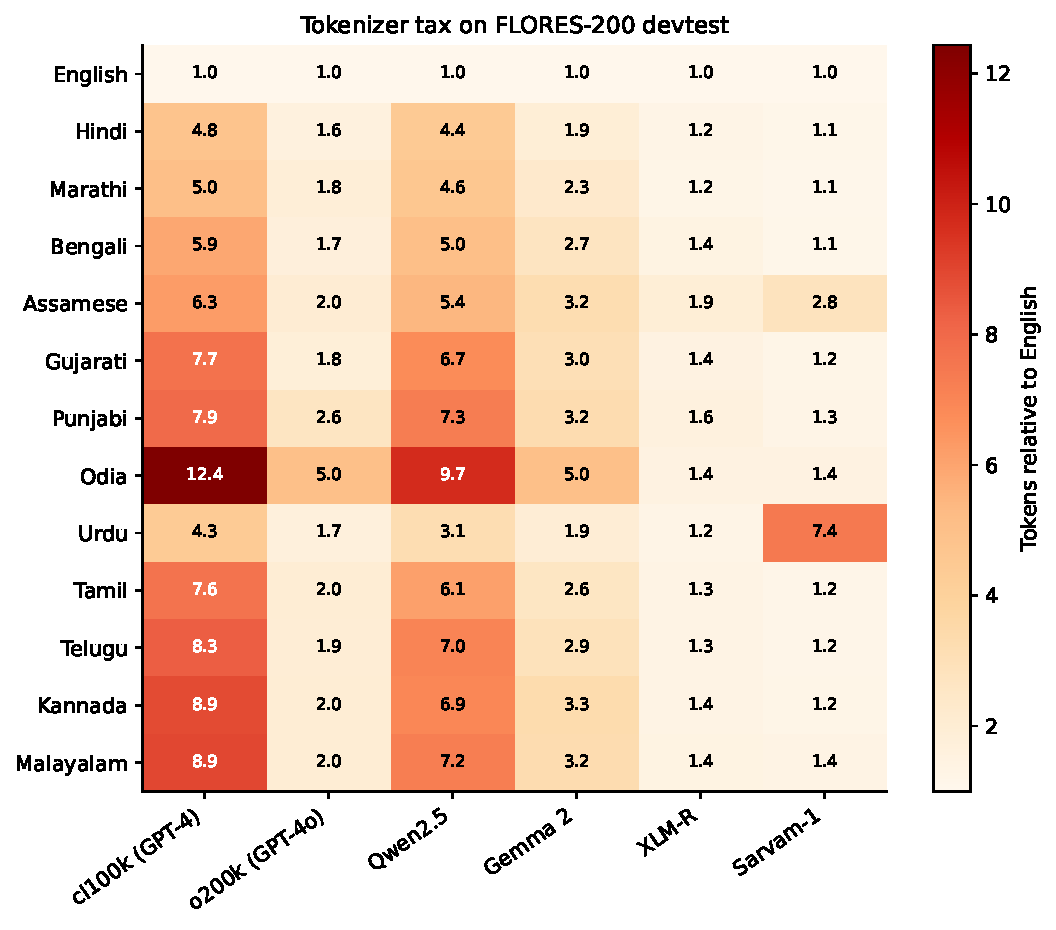
\includegraphics[width=\columnwidth]{fig_tax_heatmap}
  \caption{Tokenizer tax $T$ (tokens relative to English for the same FLORES-200 devtest content).}
  \label{fig:tax}
\end{figure}

\begin{figure}[t]
  \centering
  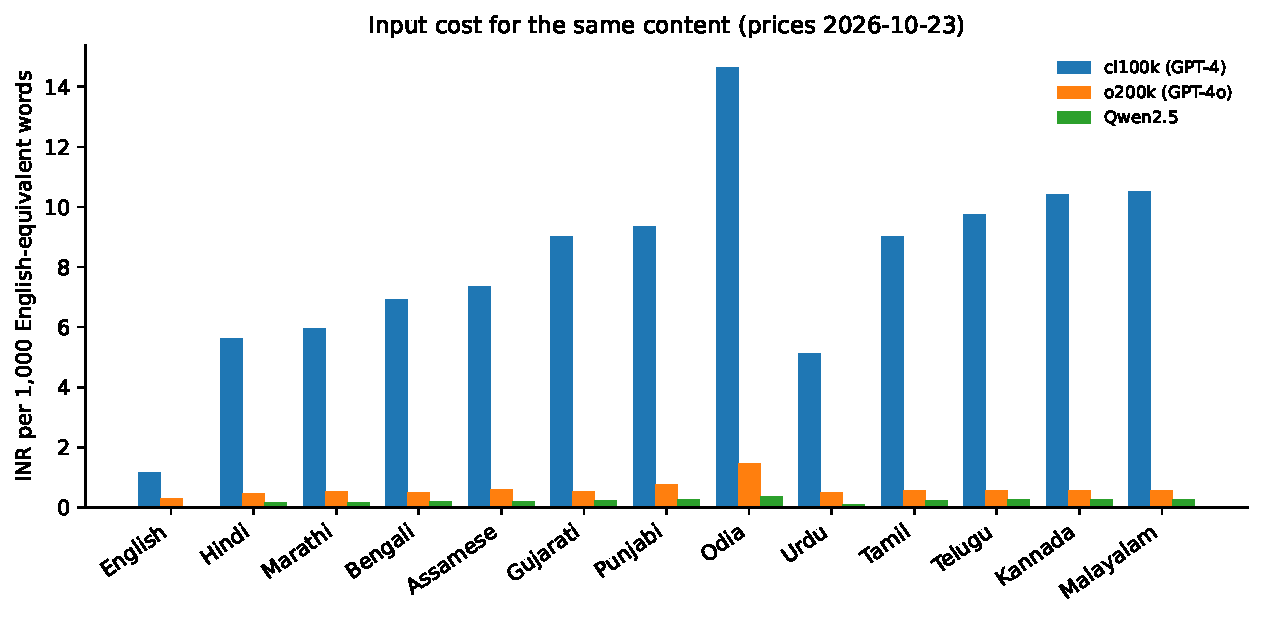
\includegraphics[width=\columnwidth]{fig_cost}
  \caption{Input cost in INR per 1{,}000 English-equivalent words at published API prices.}
  \label{fig:cost}
\end{figure}


\section{Decomposing the accuracy gap}\label{sec:method}
For model $M$, language $\ell$ and budget $B$ (the English passage's own token count), the gap
$\Delta(\ell)=A(\ell_0,\tau,B)-A(\ell,\tau,B)$ splits exactly into
\begin{align*}
\Delta_{\mathrm{ctx}} &= A(\ell,\tau,\infty)-A(\ell,\tau,B),\\
\Delta_{\mathrm{frag}} &= A(\ell_0,\tau,\infty)-A(\ell_0,s^{\ell},\infty),\\
\Delta_{\mathrm{res}} &= A(\ell_0,s^{\ell},\infty)-A(\ell,\tau,\infty),
\end{align*}
where $s^{\ell}$ re-segments each English passage until it has as many tokens as the same passage in $\ell$.
\todo{Algorithm 1 (matched fragmentation), single-byte condition, models, Belebele setup -- lanes B/C}

\section{Results}\label{sec:results}
\todo{E3 table; Figure~\ref{fig:decomp}; E4 slopes. Insert after merge day.}
\begin{figure}[t]
  \centering
  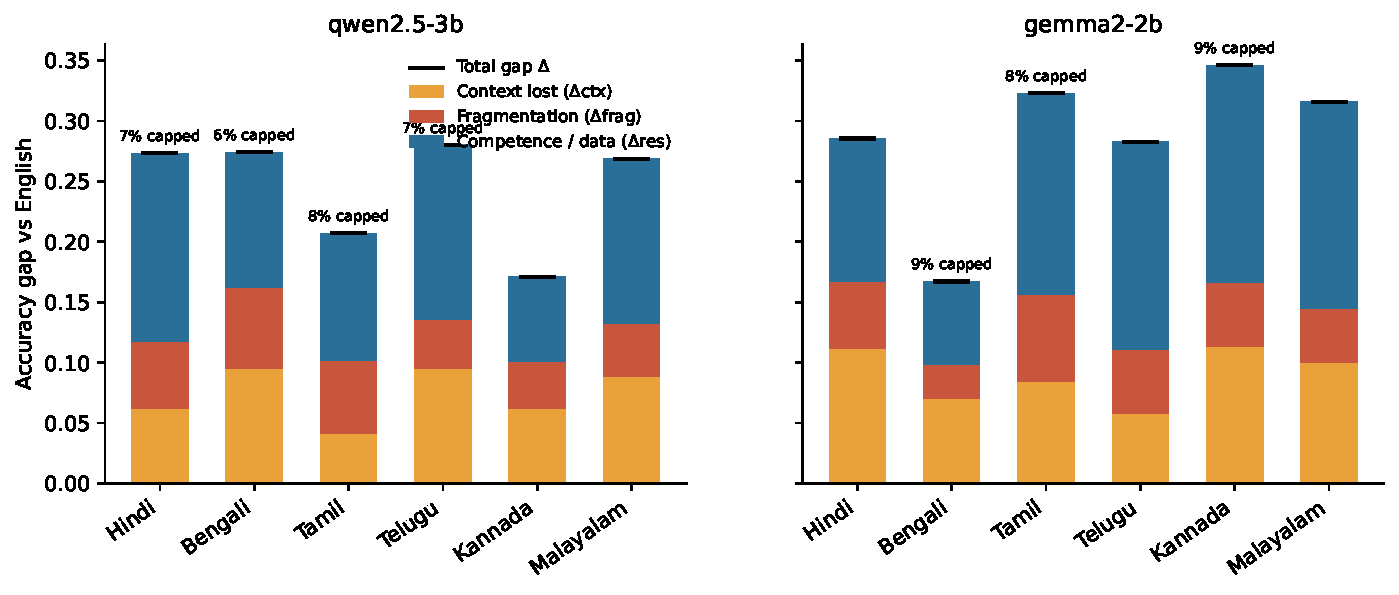
\includegraphics[width=\columnwidth]{fig_decomposition}
  \caption{Accuracy gap vs English split into context, fragmentation and competence. \todo{real data}}
  \label{fig:decomp}
\end{figure}

\section*{Limitations}
Two small (2--3B) models in 4-bit, one task (reading comprehension), 300 items per language.
Fragmented English is out-of-distribution for the model, so $\Delta_{\mathrm{frag}}$ is an upper bound.
English cannot be split finer than characters, so matching is capped for some items (reported separately).
Truncation approximates, but is not, a real long-context limit. API prices are a dated snapshot.

\bibliography{refs}
\end{document}
